\documentclass[tikz,border=8pt]{standalone}
\usepackage{amsmath}
\usetikzlibrary{arrows.meta}
\definecolor{ink}{HTML}{21352F}\definecolor{teal}{HTML}{087F7B}
\definecolor{blue}{HTML}{4B77A8}\definecolor{gold}{HTML}{C58B2A}
\begin{document}
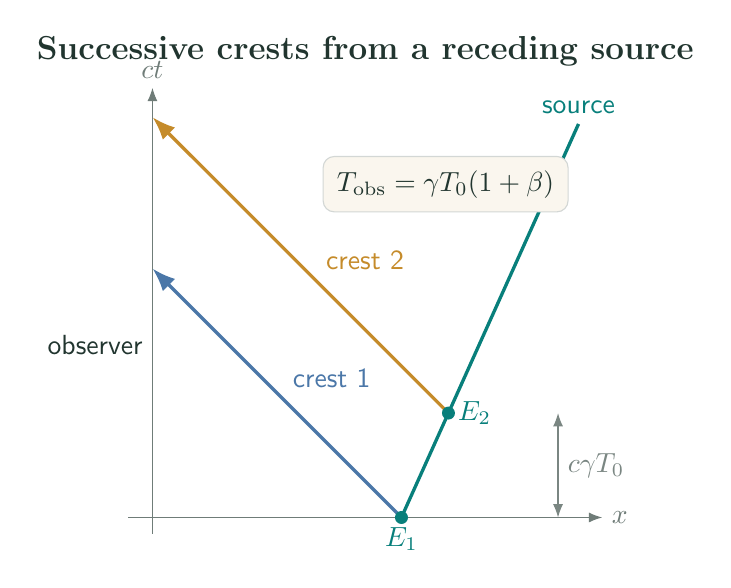
\begin{tikzpicture}[font=\sffamily,text=ink,>=Latex,scale=1.02]
  \def\bet{0.45}\def\gap{1.3}\def\xzero{3.1}
  \node[font=\bfseries\large] at (2.65,5.8) {Successive crests from a receding source};
  \draw[->,ink!65] (-.3,0)--(5.6,0) node[right] {$x$};
  \draw[->,ink!65] (0,-.2)--(0,5.35) node[above] {$ct$};
  \node[left] at (0,2.15) {observer};
  \draw[teal,very thick] (\xzero,0)--({\xzero+\bet*4.9},4.9) node[above] {source};
  \coordinate (E1) at (\xzero,0); \coordinate (E2) at ({\xzero+\bet*\gap},\gap);
  \draw[blue,very thick,->] (E1)--(0,\xzero) node[pos=.48,above right] {crest 1};
  \draw[gold,very thick,->] (E2)--(0,{\gap+\xzero+\bet*\gap}) node[pos=.45,above right] {crest 2};
  \fill[teal] (E1) circle (2.3pt) node[below] {$E_1$};
  \fill[teal] (E2) circle (2.3pt) node[right] {$E_2$};
  \draw[<->,ink!60] (5.05,0)--(5.05,\gap) node[midway,right] {$c\gamma T_0$};
  \node[draw=ink!20,fill=gold!8,rounded corners=4pt,inner sep=5pt] at (3.65,4.15)
    {$T_{\rm obs}=\gamma T_0(1+\beta)$};
\end{tikzpicture}
\end{document}
